\chapter[Introdução]{Introdução}\label{cap1}

Esse capítulo apresenta uma visão geral do projeto, como os seus objetivos e aborda acerca da inserção desse projeto em um determinado contexto. Assim esse capítulo está dividido nas seguintes seções:

\textit{Contexto} : Seção que apresenta o contexto, ou cenário, no qual o projeto está inserido.

\textit{Descrição do Problema}: Seção que descreve o problema identificado referente ao contexto apresentado.

\textit{Justificativa}: Seção que aborda uma justificativa do uso do projeto nesse contexto especificado.

\textit{Objetivos}: Seção na qual são apresentados os objetivos a serem alcançados no desenvolvimento do projeto.

\textit{Metodologia}: Seção onde é apresentada a metodologia de gerenciamento de projetos \textit{Project Management Body of Knowledge} (PMBOK), que é utilizada ao longo do desenvolvimento do trabalho.

\textit{Plano de Comunicação}: Seção que trata acerca da comunicação da equipe do projeto.

\textit{Ferramentas Computacionais}: Seção que descreve as ferramentas utilizadas na construção dos itens deste relatório e que foram utilizadas para interação entre os membros da equipe.


\section{Contexto}
  As doenças cardio vasculares fazem parte de condições que predispõe uma pessoa à maiores riscos de 
desenvolver e sofrer ataques do coração e dos vasos sanguíneos. Alguns dos fatores de risco para tais problemas são: 
hábitos alimentares ruins, fumo, obesidade, sedentarismo, diabetes e idade avançada. \cite{ceolin}

As doenças crônicas são responsáveis por mais de 72\% de mortes no Brasil. Onde o governo tem como principal arma a tais patologias, 
a prevenção. Qual age através de diversas ações para prevenir doenças cardíacas e respiratórias pelo Programa Saúde da Família a fim de promover
uma mudança de hábitos a população brasileira, contudo é necessário todo um preparo para o atendimento em casos de ocorrências, devido ao alto grau de 
complexidade do paciente.

Segundo dados provenientes do Ministério da Saúde a população Distrito Federal tem envelhecido, se encontrando em uma pirâmide etária diferente, 
apresentando uma população mais velha e suscetível a doenças crônicas, onde cerca de mais de 33\% possui algum tipo de patologia crônica. \cite{portal}

Essa população é majoritariamente urbana, possuindo cerca de 4,4\% de população rural, devido a sua localização geográfica e o planejamento prévio da cidade. 
Devido a essa grande centralização de pessoas em pequenos espaços, surge uma dificuldade de locomoção no perímetro, principalmente, em horários de pico, 
gerando diversos acidentes entre veículos, de modo que, nas localidades que ocorrem tais ocorrências, o planejamento estrutural de tráfego foi abandonado, 
tornando o socorro ás vitimas mais árduo. \cite{oliveira}

Uma solução para a dificuldade no acesso no local da emergência tem sido a utilização de um Veículo Aéreo Não Tripulado (VANT). 
De acordo com Takei (\citeyear{DEE}), o uso de VANTs tem acarretado no aumento da taxa de sobrevivência e no aumento da eficiência do sistema de pronto-socorro.
\section{Descrição do Problema}
A partir do contexto apresentado o problema a ser solucionado é:
Demora no socorro pré-hospitalar dadas as dificuldades de acesso das ambulâncias, por natureza ou por circunstância.

\section{Justificativa}
  O atendimento pré-hospitalar é o procedimento feito após a ocorrência de um agravo à saúde da vítima \cite{SBC} sendo esse um atendimento de alta complexidade, 
devido ao fato de algumas ocorrências apresentarem riscos de vida ao paciente, que requer um atendimento muito ágil e eficaz, durante a primeira hora após o ocorrido, 
podendo este ser determinante para sobrevivência do mesmo.\cite{PQA} 
As principais ocorrências de atendimento pré-hospitalar de acordo com o Corpo de Bombeiros podem ser vistas na Figura 1. Segundo esses dados aproximadamente 15\% das ocorrências atendidas são os casos de problemas cardíacos, respiratórios e hemorragias.


O tempo de atendimento à vítima de PCR (Parada Cardiorrespiratória) é extremamente importante. Receber a RCP (Ressucitação Cardiopulmonar) a tempo pode ser determinante para a sobrevivência do paciente, a cada minuto que passa a chance de sobrevivencia cai de 7 a 10\% \cite{SBC}. 
 \begin{figure}[H]
<<<<<<< Updated upstream
	\centering
		\includegraphics[keepaspectratio=true,scale=0.6]{figuras/bombeiros.eps}
	\caption[Gráfico do número de atendimentos pré-hospitalar do corpo de bombeiros]{Gráfico do número de atendimentos pré-hospitalar do corpo de bombeiros. Fonte: \cite{bombeiro}}
\end{figure}
% \vfill

O DEA (Desfibrilador externo automático) é um equipamento portátil, que interpreta o ritmo cardíaco do paciente, seleciona automaticamente o nível de energia e carrega automaticamente, e tudo que o operador precisa fazer é pressionar o botão de descarga, ele é um equipamento simples que os leigos podem usar com uma simples instrução e é de grande importância no atendimento à PCR, uma vez que grande parte delas ocorre em ambiente extra-hospitalar, como residencia e em lugares públicos \cite{SBC}.

O uso do DEA, assim que disponível, permite maior sucesso no atendimento, pois a maioria das vítimas que tem parada cardíaca em ambiente extra-hospitalar se encontra em FV (Fibrilação Ventricular) \cite{SBC}.

Dessa forma, um grande  problema  que existe em um salvamento é o deslocamento da unidade de salvamento até o local do acidente. Muitas vezes esse caminho está obstruído devido a trânsito, dificuldades de acesso como em casos de favelas e invasões ou muitas vezes locais distantes das unidades de pronto-atendimento que estão sobrecarregadas. Essa obstrução de modo geral, causa atraso no socorro.
Para chegar em locais de difícil acesso, há o uso do helicóptero, todavia seu uso envolve custos altos, alguns desses custos podem ser vistos
na Tabela \ref{tab:custos}.

\begin{table*}
\caption{Custos relacionados ao uso do helicóptero para o CBMDF. Fonte: \cite{bombeiro}}
\label{tab:custos}
\centering
  \begin{tabular}{|p{0.45\linewidth}|p{0.25\linewidth}|}
  \hline
  Descrição & Valor\\
  \hline
  Valor do helicóptero comprado em 2014 & R\$ 37.288.839,00 \\

  Treinamento de pilotos e mecânicos & R\$ 118.725,00\\
  
  Manutenção dos helicópteros & R\$ 409.886,00 \\

  \hline
  \end{tabular}
\end{table*}

O  EmerVant  vem  com a  proposta  de otimizar  o tempo  entre  a ocorrência do acidente  e a chegada  do socorro, através do uso de um VANT capaz de carregar de equipamentos que auxiliem o pré-atendimento hospitalar. 

Pinto e Cassemiro (\citeyear{pinto}) afirmam que ``A utilização de Veículos Aéreos Não-Tripulados (VANTs) tem se mostrado uma excelente alternativa, já que dispõe de uma flexibilidade maior e um custo baixo comparado às soluções tradicionais.''

Assim, esse projeto tem como objetivo solucionar os problemas referentes à socorros emergenciais que são causados pela distância entre socorristas e pacientes, realizando através de dois equipamentos e um kit, que irão ser transportados pelo VANT, procedimentos rápidos, onde não será necessária a presença física de um socorrista, e que se forem realizados no menor tempo possível, podem aumentar a chance de sobrevivência do paciente.

\section{Objetivos}
  \chapter{Desenvolvimento}\label{cap2}
 Nessa seção será apresentado o escopo do projeto e a proposta de solução.
\section{Escopo}
Para definição do escopo do projeto foram analisados os seguintes aspectos: local de atuação, situações de socorro pré-hospitalar, viabilidade dos itens a serem levados pelo VANT, elementos estruturais e planejamento e estratégia de voo do VANT e comunicação com o usuário.

\begin{description}
  \item[Local de Atuação] \hfill 
  	\begin{itemize}
  		\item Locais de difícil acesso no DF seja por natureza ou circunstância.
  	\end{itemize}
  \item[Tipo de emergência] \hfill 
  	\begin{itemize}
  		\item Parada Cardíaca
		\item Parada Respiratória
		\item Hemorragia Externa
  	\end{itemize}
  \item[Equipamentos Utilizados para salvamento] \hfill \\
  	Para definir os itens a serem levados foi realizada uma análise de viabilidade levando em consideração a utilização dos equipamentos por pessoas sem conhecimento em salvamento e a possibilidade de carga útil do VANT.
  	\begin{itemize}
  		\item Kit primeiro socorros
		\item Desfibrilador Automático
		\item Reanimador ventilatório manual
		\item Kit de hemorragias externas
  	\end{itemize}
  \item[Distância de Operação] \hfill 
  	\begin{itemize}
  		\item Haverá uma única central de controle
  		\item Velocidade máxima do drone: 70 km/h
  		\item O VANT operará em um raio de 80km. Sendo o centro do raio a ambulância onde se encontra o drone.
  	\end{itemize}
  \item[Sinais vitais que serão monitorados] \hfill 
  	\begin{itemize}
  		\item Eletrocardiograma
  	\end{itemize}
  \item[Projeto mecânico estrutural] \hfill 
  	\begin{itemize}
  		\item Asa rotatória
		\item Elétrico
  	\end{itemize}
  \item[Materiais] \hfill 
  	\begin{itemize}
  		\item Polímeros compostos
		\item Fibra de carbono
  	\end{itemize}
  \item[Controle] \hfill 
  	\begin{itemize}
  		\item Controle automático comandado pela central de comunicação. (Rádio frequência)
  	\end{itemize}
  \item[Comunicação entre equipe de paramédicos e usuário] \hfill 
  	\begin{itemize}
  		\item Câmera e sistema de áudio. Sendo que, o video será apenas para o paramédico da central e a comunicação via áudio para ambos.
  		\item O usuário apenas escutará as instruções, se comunicando apenas através do áudio.
  	\end{itemize}
  \item[Sensores] \hfill 
  	\begin{itemize}
  		\item Eletrocardiograma para medir os sinais vitais
		\item GPS - Utilizado para o deslocamento e localização do VANT
		\item Acelerômetro - Utilizado para obter uma localização mais apurada
		\item Giroscópio - Refinamento na localização
		\item Controlador A2 DJI
  	\end{itemize}
  \item[Projeto unidade central de processamento] \hfill 
  	\begin{itemize}
  		\item Controlador A2 DJI
  	\end{itemize}
  \item[Conversão e armazenamento de energia] \hfill 
  	\begin{itemize}
  		\item Bateria
  	\end{itemize}
  \item[Estimação de consumo energético e autonomia] \hfill 
  	\begin{itemize}
  		\item 4 horas de voo
  	\end{itemize}
\end{description}

\section{Estrutura Analítica de Projeto - EAP}

No desenvolvimento de qualquer projeto, é essencial ter uma visão geral sobre as atividades que serão realizadas no decorrer da processo de criação.  Para isso existem formas de sistematização e organização dessas informações.

Uma dessas formas de organizar a informação é a EAP - Estrutra Analítica do Projeto - que é a estruturação das entregas a serem completadas em forma de árvore de maneira hierárquica, onde são distribuídas da mais gerais para as mais especificas.

A EAP foi a forma escolhida pela equipe de desenvolvimento do projeto EmerVant para estruturação das entregas, por proporcionar de uma maneira simples e objetiva todos os pontos abordados e discutidos para a realização do projeto em seu devidos graus de importância. 

Para a criação da EAP do EmerVant, foi observado que dentro do projeto há varias áreas de atuação. Assim os níveis mais gerais foram definidos por essas áreas de atuação que são:
\begin{itemize}
\item Gerência de Projetos
\item Iniciação
\item Estrutura do VANT
\item Comunicação
\item Controle
\item Fonte Energética
\item Encerramento
\end{itemize}

\begin{figure}[ht]
  \centering
    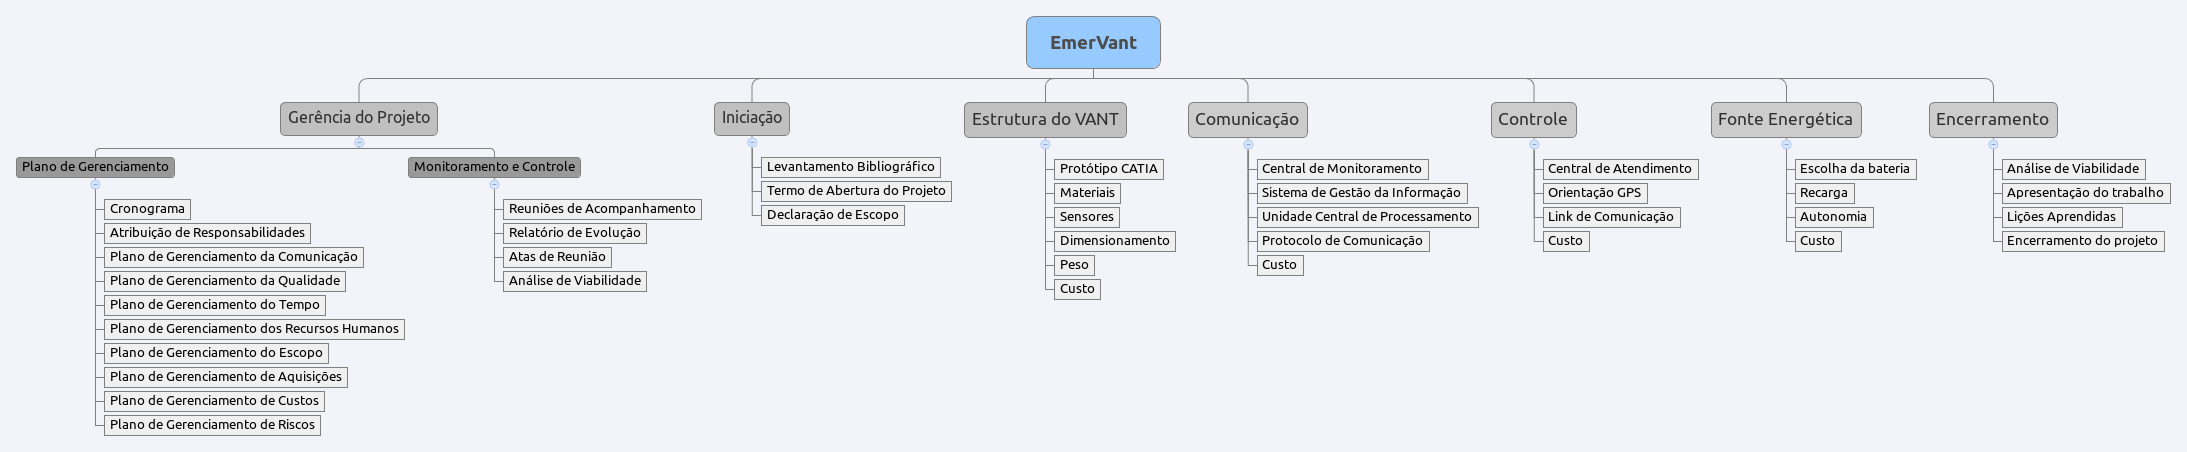
\includegraphics[keepaspectratio=true,scale=0.7,angle=90]{figuras/eap.eps}
  \caption{Estrutura Analítica do Projeto EmerVant}
\end{figure}

As entregas especificas de cada tópico foram baseadas nas definições de escopo e requisitos. A Figura 5 é a representação gráfica da EAP criada para o projeto EmerVant.

\section{Solução Inicial}
O EmerVant consiste em um sistema de assistência emergencial através da utilização de um VANT.  

O grande potencial dos drones tem sido explorado em inúmeras implementações militares e civis. Entre as vários VANTs, estes de pequena escala são especialmente atraentes para o meio acadêmico, devido ao seu pequeno tamanho, as capacidades de voo único, excelente dirigibilidade e baixo custo.\cite{SDM}

Também é possível que essas informações podem ser recebidas de fontes remotas, como GPS de satélites. Em uma situação normal o desempenho do piloto automático excede a controlada por humanos, e mesmo em situações mais desafiadoras sua performance é equivalente.

O projeto mecânico estrutural será constituído de polímeros compostos e fibra de carbono. O VANT será de asa rotatória e utilizará sistemas embarcados e sensores. O controle será feito através de um sistema automático com o uso de \textit{Global Position System} (GPS), utilizado para deslocamento e localização. 

O piloto automático deve ter acesso às informações em tempo real, e com isso computar a sua altitude, lugar no espaço e sua localização à obstáculos. Para gerar essas informações são necessários: giroscópios, acelerômetro, sensores magnéticos e eletromagnéticos, sensores visuais, infravermelhos, micro-ondas e gamas de rádio.\cite{UDE}

A partir isso, o tempo de voo foi estimado em quatro horas e o deslocamento do drone será com velocidade média de 70km/h e com raio de atuação de 80km da ambulância onde o mesmo está, a priori, acoplado. 

Esse sistema será monitorado através de uma central que receberá as informações referentes ao local e situação da(s) vítima(s) para repassá-las a ambulância e enviar as coordenadas para o VANT, que somente será ativado através da requisição da ambulância. 

O monitoramento do VANT ocorrerá através de um sistema de controle automático por rádio frequência que terá uma câmera e um sistema de áudio. 

O VANT através da câmera e do sistema de áudio estabelecerá a comunicação entre o usuário, a ambulância e a central de monitoramento. O vídeo será apresentado apenas para o paramédico da central e o áudio para a central e a ambulância. O contato do usuário será apenas com o áudio.

\section{Cronograma}
O cronograma preliminar das atividades pode ser visto na Figura 6, e o gráfico de Gantt que relaciona as tarefas com o tempo está representado na Figura 7. As atividades estão mais especificadas apenas no Ponto de Controle 1, os demais pontos de controle estão planejados de forma macro.

 \begin{figure}[ht]
	\centering
		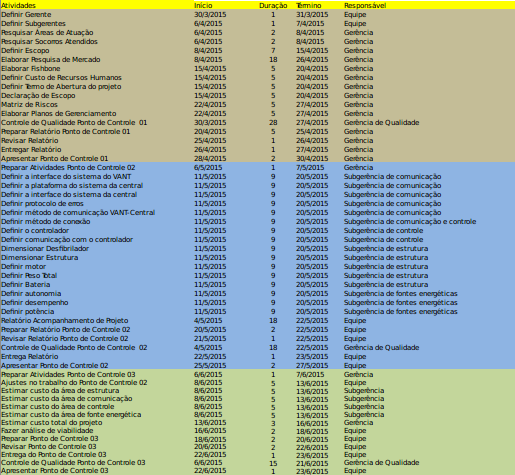
\includegraphics[keepaspectratio=true,scale=0.9]{figuras/cronograma.eps}
	\caption{Cronograma de Atividades}
\end{figure}

 \begin{figure}[ht]
	\centering
		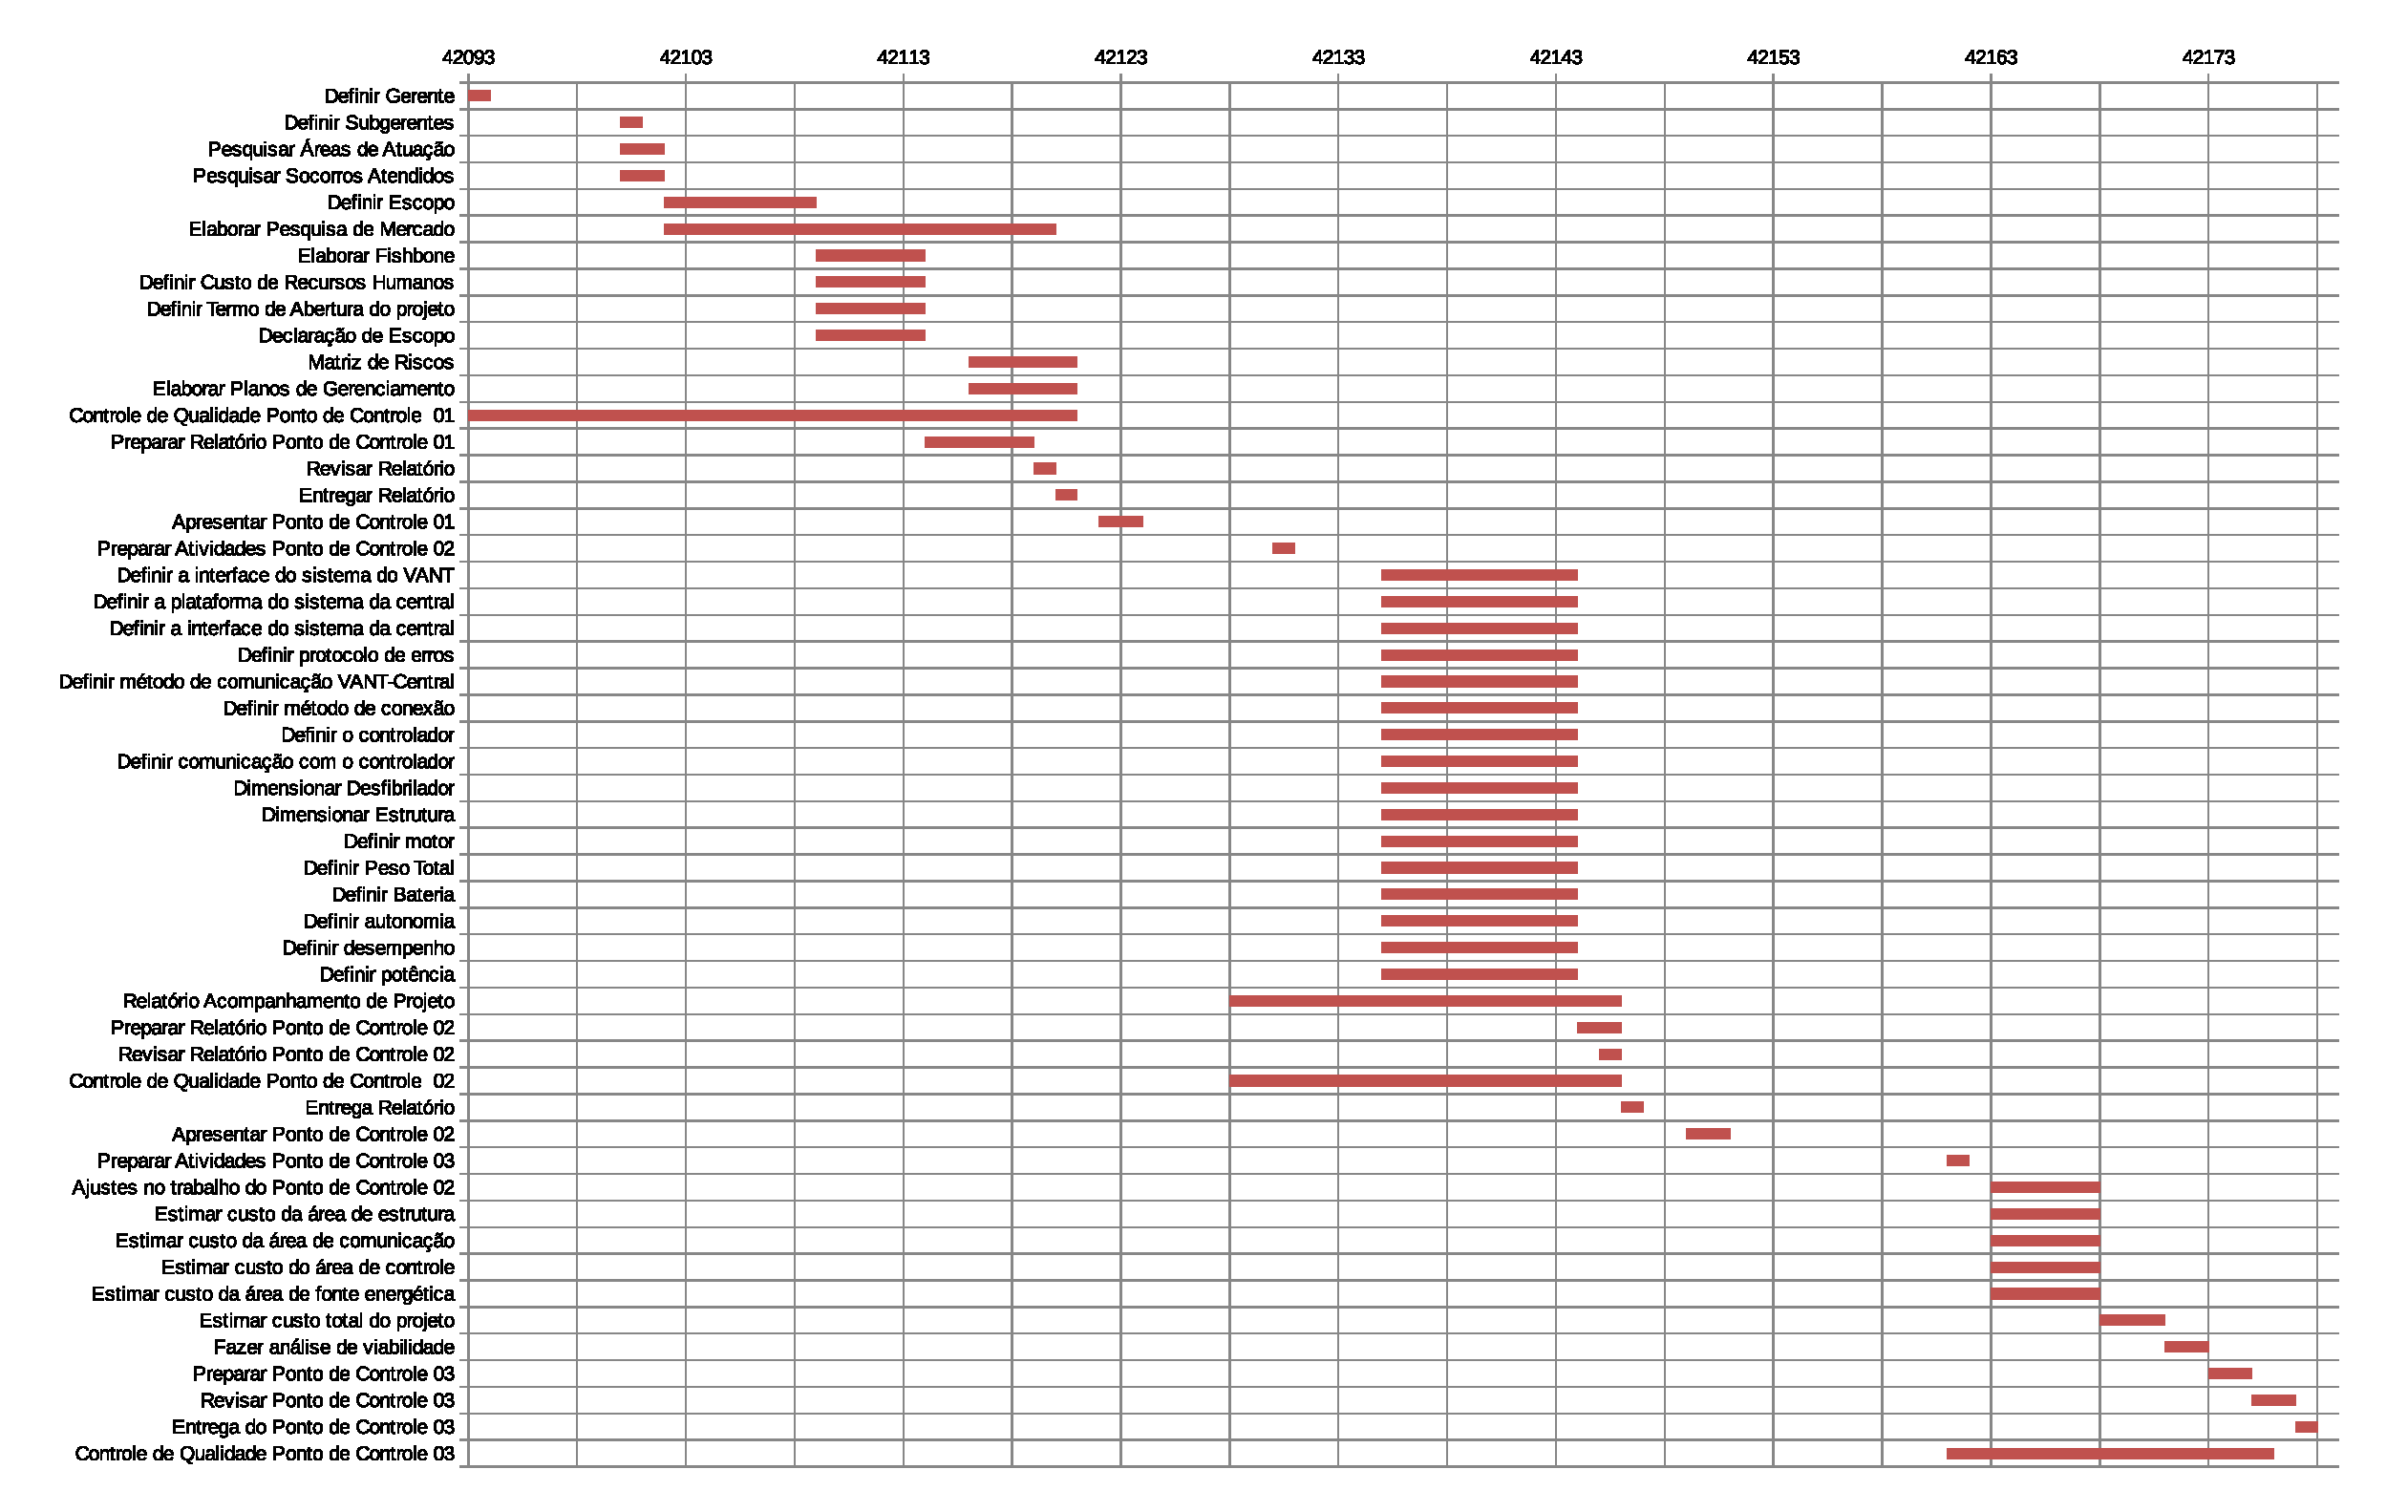
\includegraphics[keepaspectratio=true,scale=0.9,angle=90]{figuras/gantt.eps}
	\caption{Gráfico de Gantt}
\end{figure}





\section{Metodologia}
   Nessa seção será abordada a metodologia de trabalho definida para o projeto levando em consideração o seu gerenciamento e a estrutura da equipe.
\subsection{Metodologia de Gerenciamento}

Dentro das possibilidades de gerenciamento de projetos, existem duas metodologias que foram discutidas em grupo que poderiam ser adotadas para o projeto do EmerVANT, a metodologia SCRUM ou a metodologia PMBOK(Project Management Body of Knowledge). Diante do trabalho técnico que deve ser realizado e a quantidade de pessoas envolvidas, o método escolhido foi o do PMBOK porque possibilita e facilita a divisão de trabalho para grupos inexperientes, com menor capacidade variação de mudanças e cria uma cultura de controle que possibilita a elaboração de um projeto altamente crítico. Dentro do PMBOK existem nove áreas de conhecimento (Figura 2) que permitem o gerenciamento do projeto como um todo dentro das quatro estruturas da equipe que serão analisadas posteriormente.

 \begin{figure}[H]
	\centering
		\includegraphics[keepaspectratio=true,scale=0.5]{figuras/PMBOK.eps}
	\caption[Áreas de conhecimento das fases do PMBOK]{Áreas de conhecimento das fases do PMBOK. Fonte: Autores (Baseado no PMBoK)}
\end{figure}

Com o gerenciamento destas nove áreas foi possível definir diretrizes sobre o gerenciamento dos cinco grupos de processos essenciais: iniciação, execução, planejamento, controle e finalização. Os principais documentos criados a partir deste processo serão o TAP(termo de abertura), EAP(Estrutura Analítica de Projeto), plano de gerenciamento de projeto, riscos, comunicações, aquisições e estimativa de custos.

A Figura 3 mostra como funciona o fluxo detalhado das macroatividades do PMBOK e é o processo que está sendo seguindo neste trabalho:

\begin{figure}[H]
	\centering
		\includegraphics[keepaspectratio=true,scale=0.5]{figuras/pmbok-resumido.eps}
	\caption[Fluxo resumido - PMBOK]{Fluxo resumido - PMBOK. Fonte: \cite{pmbok}}
\end{figure}

\subsection{Estrutura da Equipe}
A equipe do projeto, formada por 25 integrantes, foi subdivida em quatro áreas de pesquisas, que são elas: estrutura do VANT, comunicação, controle e fonte energética. As áreas são coordenadas por um subgerente, um para cada área, e ambos são supervisionados e administrados por um gerente geral, Henrique Berilli, e uma gerente de qualidade, Emilie Morais.

A equipe responsável pela estrutura do VANT, gerenciada por Renan Santos, é responsável pelo estudo e seleção dos a serem utilizados, processo de fabricação, sensores, unidade central de processamento e custos do VANT. Esta equipe também é responsável pelo desenho 3D das peças do VANT na ferramenta CATIA.  
	
Coordenada por Leonardo Cambraia, a área responsável pela comunicação, abrangerá o projeto da central de monitoramento, sistema de gestão e informação e custos.
	
A área de controle, gerenciada por Jennifer Cavalcante, estuda a central de controle, o comando do VANT via orientação GPS (Global Positioning System) e pelo link de comunicação VANT - Central de monitoramento.
	
A quarta área, responsável pela fonte energética, e gerenciada por Bárbara Hélen, tem como responsabilidade escolher a fonte de energia, avaliar o consumo energético e autonomia e os custos.
	
A Figura 4 ilustra a estrutura de gerenciamento (hierárquica) do projeto. Foi tomado um cuidado para que nenhum componente da equipe ficasse ocioso. Nota-se que a qualquer momento algum membro poderá ser realocado de modo a melhor suprir as necessidades do projeto.

\begin{figure}[H]
	\centering
		\includegraphics[keepaspectratio=true,scale=0.5]{figuras/equipe.eps}
	\caption{Estrutura gerencial do projeto.}
\end{figure}

\section{Plano de Comunicação}
O grupo organizou o plano de comunicação em reuniões presenciais semanais. Todas as reuniões são discursões sobre a temática do projeto onde sempre há o relato, através de ata de reunião, dos assuntos e decisões tomadas. 

Reuniões presenciais predefinidas:
\begin{itemize}
	\item Segundas (16h às 18h)
	\item Quartas (16h às 18h)
\end{itemize}

Além das reuniões presenciais, há a comunicação e avisos via grupo nas seguintes ferramentas:
\begin{itemize}
	\item Facebook
	\item WhatsApp
	\item Google Drive
	\item Trello
\end{itemize}

\section{Ferramentas Computacionais}

\textbf{FACEBOOK}:
Foi criado um grupo nesta rede social contendo os 25 membros, denominado de “PI1 Grupo 4 (VANT)”. Neste grupo discutido a possibilidade de futuras reuniões extras, é compartilhado arquivos produzidos fora das reuniões, assim como referências que podem auxiliar no desenvolvimento do projeto. Enquetes são feitas para discutir assuntos gerais pertinentes ao projeto. 

\textbf{WHATSAPP}: 
Neste aplicativo os integrantes comunicam entre si de maneira direta para avisos importantes, pequenas discursões e algumas decisões que não necessitam de uma reunião presencial.

\textbf{GOOGLE DRIVE}: 
Nesta pasta online, os 25 integrantes do grupo tem liberdade para modificar e compartilhar o desenvolvimento do trabalho. Todo o material de pesquisa, atas, relatórios, imagens, questionários e planos de trabalho são disponibilizados, para que todos tenham acesso as informações de cada área, visto que todas as áreas são interligadas.

\textbf{TRELLO}:
Nesta ferramenta organiza-se de tarefas e eventos de uma forma muito dinâmica e funcional, com ela é possível dividir as atividades entre os integrantes, fazer comentários sobre cada função empregada e ter um controle sobre tudo que já foi desenvolvido, os afazeres que estão em fase de desenvolvimento e tudo que está com pendencias.

\textbf{LATEX}:
Nesta ferramenta edita-se os relatórios e resultados do projeto de uma forma mais organizada e com um layout melhor apresentável.

\textbf{CATIA}:
Computer Aided Three-dimensional interactive application - CATIA - é uma multi-plataforma CAD(Computer aided Design), CAM(Computer-aided manufacturing) e CAE(Computer aided engineering). Utilizado para prototipação do VANT em ambiente tridimencional.

\textbf{KEYSHOT}:
Software para renderização e animação de arquivos 3d. Foi utilização para renderizar o protótipo desenvolvido no CATIA.



